%!TEX TS-program = xelatex
\documentclass[12pt]{article}

\usepackage[english]{babel}

\usepackage{amsmath}
\usepackage[T1]{fontenc}

\usepackage{geometry}
\usepackage{setspace}

\usepackage[hang,flushmargin]{footmisc}

\setlength{\parindent}{0pt}
\setlength{\parskip}{6pt plus 2pt minus 1pt}\providecommand{\tightlist}{%
  \setlength{\itemsep}{0pt}\setlength{\parskip}{0pt}}

\makeatletter
\newcounter{tableno}
\newenvironment{tablenos:no-prefix-table-caption}{
  \caption@ifcompatibility{}{
    \let\oldthetable\thetable
    \let\oldtheHtable\theHtable
    \renewcommand{\thetable}{tableno:\thetableno}
    \renewcommand{\theHtable}{tableno:\thetableno}
    \stepcounter{tableno}
    \captionsetup{labelformat=empty}
  }
}{
  \caption@ifcompatibility{}{
    \captionsetup{labelformat=default}
    \let\thetable\oldthetable
    \let\theHtable\oldtheHtable
    \addtocounter{table}{-1}
  }
}
\makeatother

\usepackage{array}
\newcommand{\PreserveBackslash}[1]{\let\temp=\\#1\let\\=\temp}
\let\PBS=\PreserveBackslash

\usepackage[breaklinks=true]{hyperref}
\hypersetup{colorlinks,%
citecolor=blue,%
filecolor=blue,%
linkcolor=blue,%
urlcolor=blue}
\usepackage{url}

\usepackage{caption}
\setcounter{secnumdepth}{0}
\usepackage{cleveref}

\usepackage{graphicx}
\makeatletter
\def\maxwidth{\ifdim\Gin@nat@width>\linewidth\linewidth
\else\Gin@nat@width\fi}
\makeatother
\let\Oldincludegraphics\includegraphics
\renewcommand{\includegraphics}[1]{\Oldincludegraphics[width=\maxwidth]{#1}}

\usepackage{longtable}
\usepackage{booktabs}

\usepackage{color}
\usepackage{fancyvrb}
\newcommand{\VerbBar}{|}
\newcommand{\VERB}{\Verb[commandchars=\\\{\}]}
\DefineVerbatimEnvironment{Highlighting}{Verbatim}{commandchars=\\\{\}}
% Add ',fontsize=\small' for more characters per line
\usepackage{framed}
\definecolor{shadecolor}{RGB}{248,248,248}
\newenvironment{Shaded}{\begin{snugshade}}{\end{snugshade}}
\newcommand{\KeywordTok}[1]{\textcolor[rgb]{0.13,0.29,0.53}{\textbf{#1}}}
\newcommand{\DataTypeTok}[1]{\textcolor[rgb]{0.13,0.29,0.53}{#1}}
\newcommand{\DecValTok}[1]{\textcolor[rgb]{0.00,0.00,0.81}{#1}}
\newcommand{\BaseNTok}[1]{\textcolor[rgb]{0.00,0.00,0.81}{#1}}
\newcommand{\FloatTok}[1]{\textcolor[rgb]{0.00,0.00,0.81}{#1}}
\newcommand{\ConstantTok}[1]{\textcolor[rgb]{0.00,0.00,0.00}{#1}}
\newcommand{\CharTok}[1]{\textcolor[rgb]{0.31,0.60,0.02}{#1}}
\newcommand{\SpecialCharTok}[1]{\textcolor[rgb]{0.00,0.00,0.00}{#1}}
\newcommand{\StringTok}[1]{\textcolor[rgb]{0.31,0.60,0.02}{#1}}
\newcommand{\VerbatimStringTok}[1]{\textcolor[rgb]{0.31,0.60,0.02}{#1}}
\newcommand{\SpecialStringTok}[1]{\textcolor[rgb]{0.31,0.60,0.02}{#1}}
\newcommand{\ImportTok}[1]{#1}
\newcommand{\CommentTok}[1]{\textcolor[rgb]{0.56,0.35,0.01}{\textit{#1}}}
\newcommand{\DocumentationTok}[1]{\textcolor[rgb]{0.56,0.35,0.01}{\textbf{\textit{#1}}}}
\newcommand{\AnnotationTok}[1]{\textcolor[rgb]{0.56,0.35,0.01}{\textbf{\textit{#1}}}}
\newcommand{\CommentVarTok}[1]{\textcolor[rgb]{0.56,0.35,0.01}{\textbf{\textit{#1}}}}
\newcommand{\OtherTok}[1]{\textcolor[rgb]{0.56,0.35,0.01}{#1}}
\newcommand{\FunctionTok}[1]{\textcolor[rgb]{0.00,0.00,0.00}{#1}}
\newcommand{\VariableTok}[1]{\textcolor[rgb]{0.00,0.00,0.00}{#1}}
\newcommand{\ControlFlowTok}[1]{\textcolor[rgb]{0.13,0.29,0.53}{\textbf{#1}}}
\newcommand{\OperatorTok}[1]{\textcolor[rgb]{0.81,0.36,0.00}{\textbf{#1}}}
\newcommand{\BuiltInTok}[1]{#1}
\newcommand{\ExtensionTok}[1]{#1}
\newcommand{\PreprocessorTok}[1]{\textcolor[rgb]{0.56,0.35,0.01}{\textit{#1}}}
\newcommand{\AttributeTok}[1]{\textcolor[rgb]{0.77,0.63,0.00}{#1}}
\newcommand{\RegionMarkerTok}[1]{#1}
\newcommand{\InformationTok}[1]{\textcolor[rgb]{0.56,0.35,0.01}{\textbf{\textit{#1}}}}
\newcommand{\WarningTok}[1]{\textcolor[rgb]{0.56,0.35,0.01}{\textbf{\textit{#1}}}}
\newcommand{\AlertTok}[1]{\textcolor[rgb]{0.94,0.16,0.16}{#1}}
\newcommand{\ErrorTok}[1]{\textcolor[rgb]{0.64,0.00,0.00}{\textbf{#1}}}
\newcommand{\NormalTok}[1]{#1}

\newlength{\cslhangindent}
\setlength{\cslhangindent}{1.5em}
\newlength{\csllabelwidth}
\setlength{\csllabelwidth}{3em}
\newenvironment{CSLReferences}[3] % #1 hanging-ident, #2 entry spacing
 {% don't indent paragraphs
  \setlength{\parindent}{0pt}
  % turn on hanging indent if param 1 is 1
  \ifodd #1 \everypar{\setlength{\hangindent}{\cslhangindent}}\ignorespaces\fi
  % set entry spacing
  \ifnum #2 > 0
  \setlength{\parskip}{#2\baselineskip}
  \fi
 }%
 {}
\usepackage{calc} % for \widthof, \maxof
\newcommand{\CSLBlock}[1]{#1\hfill\break}
\newcommand{\CSLLeftMargin}[1]{\parbox[t]{\maxof{\widthof{#1}}{\csllabelwidth}}{#1}}
\newcommand{\CSLRightInline}[1]{\parbox[t]{\linewidth}{#1}}
\newcommand{\CSLIndent}[1]{\hspace{\cslhangindent}#1}
\geometry{verbose,letterpaper,tmargin=2.5cm,bmargin=2.5cm,lmargin=2.5cm,rmargin=4.5cm}
\usepackage{lineno}
\usepackage[nolists,noheads]{endfloat}

\pagestyle{plain}

\begin{document}

{\Large\bfseries Predicted interactions to iteratively update species
distribution models}
\vskip 5em
Last revision: \emph{\today}
\vskip 5em
\textbf{Abstract: }Species distribution models are characterized by
three aspects of a species occurrence: its biotic environment, its
abiotic environment, and its mobility range. Nevertheless, most
distribution models do not address the biotic interactions that
potentially shape a species range, thus measuring only how adequate an
environment is for a given population. In this chapter we discuss how we
can work towards better species distribution models without ignoring our
knowledge about ecological networks and communities' assemblage. We
suggest this can be done in seven steps: 1. careful selection of species
to be modelled; 2. performance of habitat suitability models; 3.
prediction of a metaweb which contains the selected species; 4.
prediction of local networks' structure and assessment of their
feasibility; 5. adjustment of the probabilities of occurrence based on
the probabilities of realization of networks; and 6. iteration of this
process until the differences between probabilities tends to zero. We
highlight how this can be done with the help of machine learning
techniques both to predict local networks and to update the results of
grinellian habitat suitability models. Furthermore, we point to
promising directions on the development of these techniques and the main
challenges ecologists might face in the near future.

\clearpage

\section{Authors}

Gracielle\,Higino\,\textsuperscript{1,*}\\Francis\,Banville\,\textsuperscript{2,3,4}\\Gabriel\,Dansereau\,\textsuperscript{2,4}\\Timothée\,Poisot\,\textsuperscript{2,4}

\section{Affiliations}

\textsuperscript{1}\,Universidade Federal de
Goiás\\\textsuperscript{2}\,Université de
Montréal\\\textsuperscript{3}\,Université de
Sherbrooke\\\textsuperscript{4}\,Québec Centre for Biodiversity
Sciences\\

\section{Correspondance}

\textsuperscript{*}\,\,\texttt{graciellehigino@gmail.com}

\clearpage
\linenumbers
\doublespacing

\hypertarget{introduction}{%
\subsection{Introduction}\label{introduction}}

The occurrence of a species in a given location is an encrypted message
that travels through time. It carries the species' evolutionary history,
long migration journeys, effects of other species we do not even know
that exist, and ultimately the elements that shape its, yet unknown,
future. Ecologists have been trying to decode this message with
progressively more powerful tools, since their own field notes to highly
complex computational algorithms, such as habitat suitability models.
These models were born as an attempt to model species' distribution
based on their niche, considering their occurrences as sample points of
suitable abiotic variables and their absences as sample points of
unsuitable variables. However, these observations (environmental
variables and geographic location) only unveils part of the mystery, and
the missing link are ecological interactions.

Species distribution models can be untangled in three aspects of a
species occurrence: its biotic environment - the connections it makes
with other species -, its abiotic environment - the connection it makes
with non-living resources -, and its mobility range - how far it can go
(fig.~\ref{fig:bam})(Peterson et al. 2012). The biotic environment act
on these models as potential and realized interactions, constrained or
enabled by abiotic factors, geographical conformation and migratory
ability. Nevertheless, most distribution models do not address the
biotic interactions that potentially shape a species range (or rather do
so indirectly), thus measuring only how adequate an environment is for a
given population. Because of that, they are denominated Habitat
Suitability Models (hereafter HSMs).

\begin{figure}
\hypertarget{fig:bam}{%
\centering
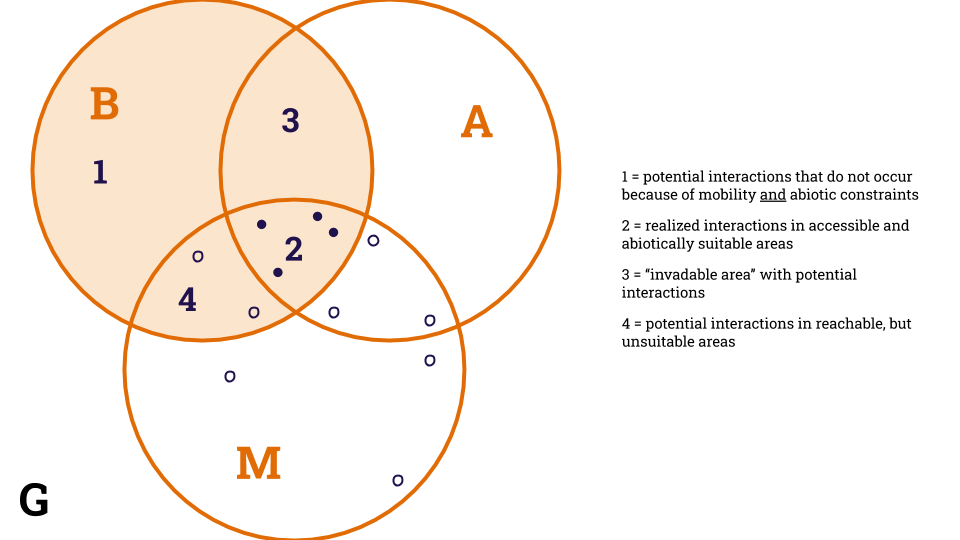
\includegraphics{figures/bam.png}
\caption{The ``BAM diagram,'' adapted from (Jorge Soberón 2007). Open
circles are absences and solid circles are observed presences. Big
circles correspond to the theoretical space of a species, regarding its
biotic interactions (the B), the abiotically suitable space (the A) and
the geographic area accessible to it (the M). These three aspects
represent real points of occurrence on the real geographic space (the
G). Ecological interactions act over this model in four ways: in (1),
there are potential interactions that are never realized because of
geographical and environmental constraints; in (2) interactions are
realized on accessible, abiotically suitable areas; the space (3) is
where the species could eventually go and establish new interactions,
while (4) is the area where the occurrence of the species is limited
only by abiotic factors.}\label{fig:bam}
}
\end{figure}

The use of HSMs is very convenient because environmental variables and
geographic limits are not (highly) dynamic variables from the
evolutionary point of view. Because the climate (used to) change at a
very slow pace, as well as species' niche, we could expect to find the
same pool of species that are able to live in a certain region, even if
populations fluctuated at a smaller temporal scale. This is because the
cumulative effect of small scale variation on climate, population
dynamics and habitat suitability itself results in macroecological
outcomes such as combinations of extinction and cladogenesis, which lead
to biodiversity distribution at continental scales. Also, abiotic
variables are not under the influence of the focal species, which make
them statistically safe, and their relationship with the species' niche
is assumed to be static in space and time, which adds generalization to
the model. The biotic space, on the other hand, is usually highly
dynamic and variable, and it can be stochastic at very small scales to
predictable structures at large scales. Additionally, because ecological
networks are the cumulative result of local events (Poisot and Stouffer
2016; Guimarães 2020), its properties can vary with environmental
factors and species evolutionary history (Martín González et al. 2015;
Dalsgaard et al. 2013).

There is a big ecological and evolutionary leap between local dynamics
of species and the biogeographical processes that are the primary
assumptions to the habitat suitability and species distribution models.
However, because ecological networks are very informative and aggregate
populations' dynamics through scales, it is conceptually important to
include them in HSMs. In fact, it has been shown that HSMs are more
efficient when ecological interactions are accounted for (either
directly or indirectly) (Wisz et al. 2013; Cazelles et al. 2016). Some
strategies have been adopted by the scientific community to accomplish
that and are shortly reviewed later in this paper. Correlative
approaches assume that the co-ocurrence of related species accounts for
interaction, while mechanistic models try to refine this assumption by
species traits and phenology. Currently, the scenario of habitat
suitability models accounting for the biotic environment is either too
generalistic (correlative approaches) or too precise (mechanistic), in
the sense that they only work when we have a good amount of information
about that specific species. However, empirical data on ecological
interactions are scarce, and, on the other hand, we cannot just assume
that two species will always interact when they co-occur. How could we
find balance and go further?

The good news is that ecologists have been developing techniques to
predict and forecast the ecologically realistic number of links
(MacDonald, Banville, and Poisot 2020), the nature of ecological
interactions (Elmasri et al. 2020), and networks' properties with good
accuracy. These techniques can mitigate the large and biased eltonian
shortfall that we have now (Poisot et al. 2020; Hortal et al. 2015). In
this context, we can envision an integrative approach of species
distribution modelling combined with network prediction resulting in a
more realistic, yet generalist, model where the predicted networks
update the probabilities of occurrence computed by an HSM. In this paper
we invite you to envision better species distribution models, which do
not ignore our knowledge about ecological networks and communities
assemblage. Here we suggest this can be done with the help of machine
learning techniques both to predict local networks and to update the
results of grinellian HSMs. We point to promising directions on the
development of these techniques and main challenges ecologists might
face in the near future.

\begin{figure}
\centering
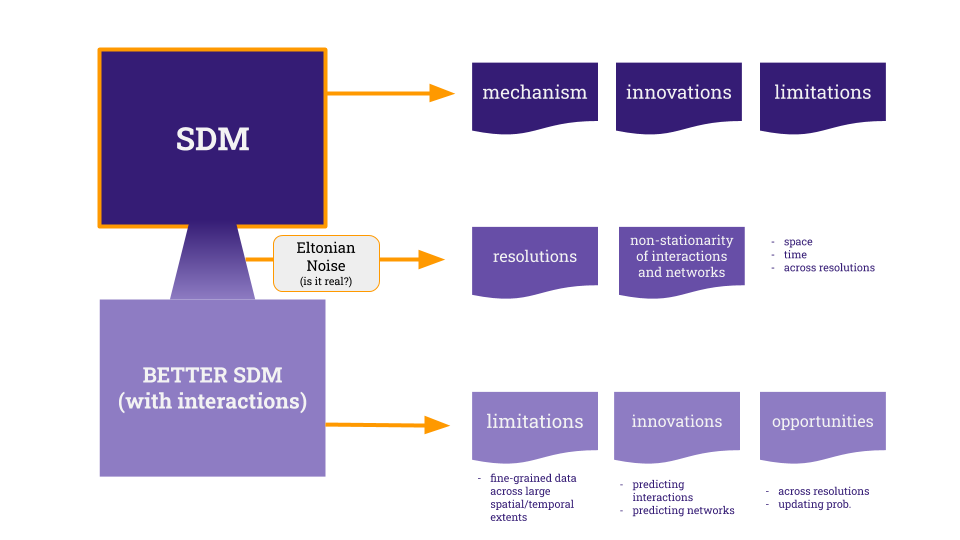
\includegraphics{figures/concept.png}
\caption{TODO}
\end{figure}

\hypertarget{hsms-the-mechanics-innovations-and-drawbacks}{%
\subsection{HSMs: the mechanics, innovations and
drawbacks}\label{hsms-the-mechanics-innovations-and-drawbacks}}

Habitat suitability models aim at finding relationships between the
occurrence of species and their environment (Guisan and Zimmermann 2000;
Guisan, Thuiller, and Zimmermann 2017). The reader might have
encountered different terminologies in this area, such as species
distribution modelling and ecological niche modelling, that supposedly
have the same objectives. The terminology is a matter of debate on the
scientific community, and here we chose to distinguish habitat
suitability models from species distribution models.

Ecological niche models and habitat suitability models focus on the the
area of A of the BAM diagram fig.~\ref{fig:bam} where a species can
occur, which means they calculate the fundamental niche of species
(Peterson et al. 2012). This can be achieved by finding the relationship
between environmental conditions and the presence or absence of a
certain species. This relationship can be static or dynamic in space,
and only makes sense when calculated for the area inside M. Therefore,
this means that they will find suitable areas inside the area 2, where
species really are, but can also find suitable areas in 5, where the
species probably are not because of biotic unsuitability. Species
distribution models, on the other hand, should aim at modelling 2 (B
\(\cap\) A \(\cap\) M), which means considering biotic constraints
(Peterson et al. 2012). Although they rarely do so, Guisan and
Zimmermann (2000) argue that the observation data used as input on these
models carries these information: when we use the physiological limits
of a species as a variable to be correlated to the environment, we are
modelling its fundamental niche, while using observational field
occurrence data implies that we are modelling the realized niche (thus,
the species distribution) because these data implicitly accounts for
biotic limitations (Guisan and Zimmermann 2000). However, because the
biotic constraints are not explicitly considered in the models, it is
possible that the predicted distribution area reaches places with
completely different communities. Because we did not consider previous
knowledge about species interactions, how can we interpret this result?
Given these differences between SDMs and HSMs, many statistical
approaches can be used to model both of them. Here we focus on the most
innovative algorithms to find the species' suitable habitats, to further
develop ideas on how to integrate biotic constraints.

Habitat suitability models are built over five steps: conceptualization,
data sampling, calibration, evaluation and prediction (Guisan, Thuiller,
and Zimmermann 2017). The conceptualization is related to the core ideas
of niche, as illustrated in fig.~\ref{fig:bam}, but also to the main
goals of the investigation. What processes are important to the patterns
we a dealing with, what is the frequency in which they repeat in space
(determining the grain and extent of the environmental variables) and
what are the direct and indirect predictors are examples of questions
that should be asked at this step. The answers to these questions will
determine how the data should be sampled (the spatial scale of the
variables) and the appropriate selection of the variables (Guisan and
Zimmermann 2000). Then the actual building of the mathematical model
enters the stage, with iterative adjustments to capture its variations.
The data is separated in training validation sets, and then the model is
used to predict and project probabilities is space that can be
interpreted as habitat suitability.

While statistical inference is a telescope that allows us to investigate
the past of biodiversity structure, machine learning algorithms are some
of the time machines we use to assess the past in order to predict the
future. They have the power to learn from the data, identifying
structure and generating predictions (Olden, Lawler, and Poff 2008). One
sound advantage of these models compared to statistical inference is
that they allow us to explore ``mischievous'' data, embracing the
multiple frequency distributions we find in nature. Many of them have
become popular among ecologists, such as MaxEnt (Phillips, Anderson, and
Schapire 2006) and Random Forest (Breiman 2001), while making a good
match with the continuously growing amount of biodiversity data.
Although these models call for cautious usage for their complexity (and
hard to interpret outputs) (Rangel and Loyola 2012), it also demands
some ecological knowledge about the relationships being modelled and
careful parameterisation of terms. These very characteristics are the
ones that allow us to explore nuances of biodiversity relationships,
such as the role of ecological interactions in shaping species
distribution - i.e.~putting the B back in the BAM model.

However, these time machines need a past to learn from, and the lack of
information about species interactions makes this past quite blurry.
Ecological interactions occur across taxonomic and geographic scales
(Guimarães 2020), and the task to collect these information through
large extents and in fine grain (both temporal and spatial) is daunting.
In addition, it is known that networks vary with climate, in space and
with phylogenetic distance {[}Poisot, Stouffer, and Gravel (2014);
CITATIONS{]}. Despite the dynamic nature of networks' structures (that
are predictable outcomes of common processes), methods such as stacked
(S-SDMs) and joint Species Distribution Models (JSDMs) are very common
to address the influence of one species over another {[}CITATIONS{]}.
These methods assume that, if a pair of species are known to interact,
they will always do so once they co-occur {[}CITATIONS{]}. For example,
in order to do a stacked SDM, one can model the assembly as a single
unit, use the predicted distribution of each species and pile them up
together, or model species at the same time, but as separate units
(Ferrier and Guisan 2006). On the other hand, JSDMs use a hierarchical
regression model to calculate the probability of occurrence of all
species together in response to environmental variables (Pollock et al.
2014). Both approaches can be considered great advances regarding
previous methods that simply added the distribution of one or more other
species as limiting factors in the model {[}CITATIONS{]}. S-SDMs and
JSDMs try to incorporate another level of complexity by modelling
assembly rules as an intermediate step towards more realistic HSMs (see
Zurell et al. (2020) for a comparison between both methods).
Nevertheless, our time machines can take us even further and incorporate
actual species interaction and predicted network properties in species
distribution models.

\hypertarget{going-further}{%
\subsection{Going further}\label{going-further}}

Spatially structured co-occurrence can be the result of many historical
and geographical processes, such as environmental heterogeneity and the
similarity of environmental preferences between species (Bar-Massada and
Belmaker 2017). HSMs that account for co-occurrence as a proxy for
interactions might wrongly capture these processes as biotic
interactions (Blanchet, Cazelles, and Gravel 2020). An important
analysis to be made before going further is at which scale ecological
interactions influence the distribution of species. Although empirical
evidence exists that ecological interactions are important processes on
population arrangements in space {[}CITATIONS{]} and networks variation
can be detected in macroecological scales {[}CITATIONS{]}, their precise
relationship with spatial scale remains unclear. A second challenge is
to deal with highly dynamic properties of ecological interactions. How
can we account for dependency between local processes in macroecological
scales? We argue that Artificial Intelligence (AI) tools can help us
identify structure on the available data and predict interactions and
networks for communities we did not access yet.

\hypertarget{the-eltonian-noise-paradox}{%
\subsubsection{The Eltonian Noise
paradox}\label{the-eltonian-noise-paradox}}

The Eltonian Noise Hypothesis states that the effect of ecological
interactions on species distribution is captured at coarse resolution
analyses as a covariation with environmental factors (Soberón and
Nakamura 2009). This logic reverts as an assumption that always that two
given species co-occur, they will interact, which has been demonstrated
to be not true (Blanchet, Cazelles, and Gravel 2020). In fact, the
contrary is likely to be true: the nature of interactions happening at a
given location affects co-occurrence (Bullock et al. 2000; Chesson and
Kuang 2008; Godsoe and Harmon 2012; Svenning et al. 2014; Godsoe et al.
2017), and they vary in space and time due to climate change,
phylogenetic diversity (addition or extinction of clades in the
community, for example)(Davies and Buckley 2011), population density
(Carnicer, Jordano, and Melián 2009), and many other factors.
Additionally, analyses of range expansion rates - a common and very
important application of HSMs - are intrinsically connected to
interspecific interactions at the border of the ranges: the expansion
tends to be slower when generalists predators are present or when
mutualists are absent (Svenning et al. 2014). On the other hand, range
preservation is also associated with ecological interactions, once
connected species can be protected of climate change and invasion
(Dunne, Williams, and Martinez 2002; Memmott, Waser, and Price 2004;
Ramos-Jiliberto et al. 2012).

This hypothesis also seems to find no support when we investigate the
betadiversity of links in ecological networks. In parasite-hosts systems
in Eurasia, it is possible to detect a distinct difference in
interactions between shared species in macroecological scale, suggesting
an ``unpacking'' of species when biodiversity is expected to be lower
{[}CHAPTER 1{]}. In addition, it is likely that species with larger
ranges of distribution and those that are more generalists would
co-occur with a greater number of other species (Dáttilo et al. 2020),
while dispersal capacity of competitive species modulate their
aggregation in space and the effect of interactions on their range
limits (Godsoe et al. 2017).

Certainly, the exact macro scale effect of interspecies interactions
might depend on the nature of these interactions, the system being
studied and the combination of geographical and environmental factors.
Younger communities may be more affected by environmental limitations,
once they are dominated by generalist species, while older
metacommunities are probably affected in different ways in the centre of
the distribution, at the edge of ranges and in sink and source
communities. In fact, there is a growing number of evidence
demonstrating that biotic interactions are important factors modulating
range shift and expansion due to rapid climate change (where
evolutionary processes are ignored, assuming that species will not have
time to adapt) (Bullock et al. 2000; Hellmann, Prior, and Pelini 2012;
Afkhami, McIntyre, and Strauss 2014; Godsoe et al. 2017; Sirén and
Morelli 2020).

Modelling species distribution considering the Eltonian Noise Hypothesis
to be true can be very useful to understand general structures of
biodiversity. At coarse resolutions, with dubious quality and sparse
data, and when the space for error is large, these models are probably
the best we can do. However, no species is an island and we should go
further whenever possible, investigating whether and how ecological
interactions exert important pressures on species ranges and spatial
arrangements. This will help us avoid spurious inferences, especially
when these models aim at conservation strategies. Fortunately, the data
we need to do that has been increasingly available (König et al. 2019),
and technologies to deal with them (with their biases and gaps) are
following.

\hypertarget{non-stationarity-of-interactions-and-networks-in-space-time-and-across-resolutions}{%
\subsubsection{Non-stationarity of interactions and networks in space,
time and across
resolutions}\label{non-stationarity-of-interactions-and-networks-in-space-time-and-across-resolutions}}

Ecological interactions are dynamic entities of ecosystems that vary in
space and time. The reason for this fluctuability is a combination of
factors that shape the probability of interactions: environmental
changes that affect the metabolism of individuals and the abundance of
populations (Rall et al. 2012; Poisot, Cirtwill, et al. 2016; Muola et
al. 2010), changes in habitat (Tylianakis and Morris 2017), and the
phylogenetic structure of communities (Coelho, Rodrigues, and Rangel
2017). Notably, the variation in traits distribution (including
phenological mismatches) are important drivers of variation in species
interactions {[}CITATIONS{]}.

Ecological networks reflect these dynamics, and, as a result, varies in
space not always in the same fashion that species richness do (Poisot,
Stouffer, and Gravel 2014). The non-stationarity of ecological networks
and their relationship with the environment can be measured and have
been demonstrated in the last few years. Dalsgaard et al. (2013) found
that modularity can be reduced and nestedness increased due to climate
change speed (Dalsgaard et al. 2013). The phylogenetic diversity of
networks is affected by dispersion and speciation rates (Coelho,
Rodrigues, and Rangel 2017; Sebastián-González et al. 2015; Trøjelsgaard
and Olesen 2013), characteristics highly correlated to both traits and
geographical structure of the environment. These examples illustrate how
networks can vary both in space (due to environmental filtering of
species traits, for example) and time (due to evolutionary changes and
phenology).

Interestingly, because ecological networks are the cumulative pool of
local interactions, it is possible that network structure varies across
scales (Galiana et al. 2018). For example, increased species richness
can promote species packing and specialization of interactions at local
scale even for generalist species {[}CITATIONS; CHAP 1{]}. Moreover, the
local combinations of species and interactions in a community can result
in very different regional pictures, since interactions can affect one
another. For example Sanders and Van Veen (2012) observed that the
persistence of two species of wasps separated by four trophic links are
conditioned to one another because they regulate the population of
competitive aphids (Sanders and Van Veen 2012). The replacement of one
species in this network can result in the local extinction of another,
even if they are not directly linked, and this dynamic could be easily
misinterpreted in regional scales as an environmental constraint.

All these peculiarities about ecological interactions and networks can
be faced as challenges or opportunities for the next years. Once we
understand how and where interactions are important to the accuracy of
species distribution models, we can use the dynamics described here as
refinements on our models. On the other hand, some of these mechanisms
act at a scale so small that stochasticity takes the stage and can be
accounted for in the error term of most models. This trade-off
reinforces the need to carefully adjust distribution models according to
the system being studied.

\hypertarget{why-we-can-go-further}{%
\subsubsection{Why we can go further}\label{why-we-can-go-further}}

A combination of global efforts and technology can make us take another
step in combining species occurrence data and ecological interactions.
In the last decades we have witnessed an increase in biodiversity data,
including citizen-science projects (Pocock et al. 2015; Callaghan et al.
2019) and organized dedicated databases mostly accessed by specialists,
such as mangal and GBIF (Poisot, Baiser, et al. 2016; {``GBIF,''} n.d.).
These data frequently describe the occurrence and the taxonomic identity
of a species, but they also capture real-time interactions (Roy et al.
2016; Ryan et al. 2018). Moreover, both occurrence and interaction data
share common characteristics that can be learned and subsequently
inferred. Because species occurrence are subject to their evolutionary
history that shaped their ecological niche, one can roughly infer where
it could occur only based on known occurrence point locations (that is
how HSMs work, as described earlier in this paper). This is connected to
how ecological networks also show signs of common ancestry and preserve
a basic structure (Riva and Stouffer 2016; Dallas and Poisot 2018). The
ever-growing number of available data and detectable structure on
ecological networks are the main ingredients we need to develop
mathematical models capable of learning from what we already know to
predict what we do not know yet.

\hypertarget{filling-in-eltonian-gaps-with-mathematics-predicting-interactions-networks-and-doing-it-across-scales}{%
\paragraph{Filling in eltonian gaps with mathematics: predicting
interactions, networks, and doing it across
scales}\label{filling-in-eltonian-gaps-with-mathematics-predicting-interactions-networks-and-doing-it-across-scales}}

A complete assessment of ecological interactions is even more difficult
than sufficient sampling of biodiversity. The number of interactions
sampled will always be lower than the number of possible interactions,
mainly due to the existence of forbidden links (Jordano 2016). This lack
of information, known as the Eltonian Shortfall, is aggravated by biases
and differences in sampling methods (Hortal et al. 2015). Nevertheless,
in the same way as the knowledge about the natural history of organisms
help us validate HSMs, understanding a species' behaviour, traits and
phylogenetic relationships can help us identify if the lack of links
sampled is due to insufficient effort or natural mismatch between
species. Additionally, interactions vary in space and time, which adds
to the uncertainty of an unregistered interaction. Hence, rather than
assuming interactions to be binary variables, we can think of them as
probabilities (Poisot, Cirtwill, et al. 2016). In fact, assuming
interactions as probabilistic events is more of an opportunity than an
obstacle. Once we understand what is the basic mix than can result in a
connection between ecological units (from individuals to ecosystems), we
can use probabilities to estimate the likelihood of our ideas even when
data is lacking. Usually, this basic mix is composed by abundance,
co-occurrence in space and time (conditional to a given environment),
and traits matching {[}Poisot, Stouffer, and Gravel (2014);
CITATIONS{]}. The regional pool of interactions also plays an important
role on interactions realization through indirect effect (Sanders and
Van Veen 2012; Poisot, Stouffer, and Gravel 2014), but they also add
another layer of complexity in predictive models.

When we do not have information about any of these properties,
interactions tend to behave as stochastic elements in our model, while
the more information we have, the more our equations will look like a
niche model. Maybe one of the most neutral approaches to predicting
interactions is assuming that two species will always interact once they
co-occur. On possible step forward is to account for spatial structure
of species distribution: interactions are more or less likely to occur
according to the location of the population inside the species range
(Svenning et al. 2014; Godsoe et al. 2017; Bar-Massada and Belmaker
2017). Moving away from stochasticity a little bit, Canard et al. (2012)
illustrates how we can build neutral networks based on species abundance
and richness, and found that the emergent properties of these networks
are compatible with empirical ones. With this method, it is possible to
identify neutral forbidden links (Canard et al. 2012), which unfolds
many other questions that can be answered without previous empirical
data. For example, we can investigate whether abundance fluctuation is
the main driver of betadiversity of links between networks, or compare
how networks are different from the neutral model when only the traits
vary. It is important to notice, however, that abundance also plays a
role on the nature of the interaction. Mutualistic interactions, for
example, can turn into parasitism or competition when one of the players
is very abundant (Wolin and Lawlor 1984).

An intermediate step could be to find detectable interactions in a
species pool. Xiao Fu et al. (2019) proposed a combination of a Poisson
N-mixture model and collaborative filtering to predict potential links
under imperfect detection. This machine learning model allowed them to
successfully infer interactions based on a few observed occurrences
sampled in the field (Xiao Fu et al. 2019). This approach deals with
interactions as countable units, ignoring evolutive and ecological
mechanisms that could lead do variation in the probability of their
realization. However, it can be a good exploratory method to investigate
the completeness of interaction sampling.

On our way to more mechanistic models, we can start looking for
evolutionary clues on our encrypted message. First, we can assume that
similar species will interact in similar ways with their ``pairs'' due
to phylogenetic inertia (Gómez, Verdú, and Perfectti 2010; Peralta
2016). If predators \emph{A} and \emph{B} are closely related, they are
likely to compete for the same set of preys. In this sense, we can use
machine learning algorithms to find in the ``potential interactions''
pool those that are more ecologically likely to occur. For example,
Desjardins-Proulx et al. (2017) showed that the \emph{K} nearest
neighbour (KNN) and the Random Forest (RF) algorithms are complementary
when it comes to identifying the probability of a predator to interact
with a certain prey and binary occurrence of interactions (RF predicts
either interaction or non-interaction) (Desjardins-Proulx et al. 2017).
According to the authors, the usefulness of these methods depend on the
kind of data we have in hands: KNNs need previous information about
interactions to learn from, while RFs should use a set of traits.
Another example of link prediction based on trait matching is Dallas,
Park, and Drake (2017), where the authors identified cryptic
associations between hosts and parasites based on a Bayesian model.
Similar to the approach on Xiao Fu et al. (2019), this model also allow
us to investigate the completeness of interaction sampling, but now
based on traits matching and not only on occurrence observations.
Pichler et al. provide an extensive methodological comparison of Machine
Learning models to predict interactions based on traits matching.
Nonetheless, these techniques isolate interactions from their biotic and
abiotic environments, and this should be kept in mind whenever
predictions are made.

Another step further would be implementing evolutionary models in the
relationship between links and phylogeny. Elmasri et al. (2020) point
out that recent approaches to link prediction using phylogenetic
similarity assume a linear or fixed diversification rate. They proceed
to develop a phylogenetic matching model of predicted interactions using
the early-burst tree scaling model, where the traits diversification
tree is transformed, adjusted by a single parameter, either to early or
late diversification (Harmon et al. 2010; Elmasri et al. 2020). The
authors also accounted for uncertainty in unobserved interactions, which
improved the accuracy of the predictions. The adjustment of the
early-burst parameter can be based on ecological reasoning. For example,
food webs with species clustered in trophic levels (specialized
predators, for example) seems to have a trait evolution with a high
diversification rate early in the tree, while networks with many
omnivorous species are thought to have a late diversification of traits
(Ingram, Harmon, and Shurin 2012). These predictions are highly
mechanistic, accounting for evolution and ecology of interactions.

Connected to the Eltonian Shortfall described at the beginning of this
session, there are global gaps and biases on network sampling (Poisot et
al. 2020). Because ecological networks are made of nodes and edges, and
both can be treated as probabilities (addressing the occurrence of a
node and the realization of an interaction), we can investigate the
chances of different networks to emerge from a set of species
co-occurring in a given location (Poisot, Cirtwill, et al. 2016).
Recently, MacDonald, Banville, and Poisot (2020) demonstrated how we can
estimate the number of possible links in a network based on the number
of species it has, which take us closer to predict networks themselves
since we have much more information about species than we have on
interactions (MacDonald, Banville, and Poisot 2020). Knowing the number
of possible links given the species richness in a given location allow
us to calculate the probability distribution for each network property,
which can be further connected to what we know about the relationship
between networks' properties and species spatial distribution

One question that is frequently stressed by macroecologists is how to
connect local processes, such as interactions, to large scale
biodiversity structures. The sampling of both interactions and
environmental variables are usually made in opposing ends of spatial
resolution, which makes them incomparable from a statistical point of
view (Peterson et al. 2012). Also, because of the nature of the
sampling, it is hard to transform those variables to make them vary in
compatible scales. How can we deal with this problem when predicting
interactions and networks for macroscales? In fact, the basic mix
components that leads to the occurrence of an interaction varies with
the spatial resolution in which it is assessed. Consequently, the
distribution of probabilities for interactions and network properties
would change, possibly leading to different interpretation of
biodiversity distribution. However, the different ways in which networks
properties vary through scales have also been investigated, and
simulations can help us understand that more deeply (Poisot, Stouffer,
and Gravel 2014; Peralta 2016; Guimarães 2020). \emph{Because}
interactions vary more in space than species occurrence (while adding to
this information) (Poisot et al. 2017), they can represent biodiversity
with a more useful macroecological variance to interplay with
environmental variables. Moreover, because interaction predictions
accounts only for \emph{potential interactions}, they are easily
translated into regional networks (that also represent potential
interactions). Finally, some properties of networks are correlated to
the phylogenetic diversity of communities {[}CHAP 1{]}, which also
represents a level of organization compatible with the geographical
scale of environmental variables.

\hypertarget{updating-probabilities-of-occurrences-with-network-probabilities}{%
\paragraph{Updating probabilities of occurrences with network
probabilities}\label{updating-probabilities-of-occurrences-with-network-probabilities}}

At this point the reader may be wondering how probabilistic networks and
species distribution models fit together. Some efforts in this sense
have already been made, and in this session we will quickly review them
while pointing to future directions. We will not consider, however, the
majority of papers that aim at discussing the integration of biotic
interactions on SDMs because their definitions of ecological
interactions are not compatible with our view. Usually, these
discussions consider the mere addition of the occurrence of a competitor
or mutualist species as a predictor variable on the model to be
sufficient to account for ecological interactions {[}Guisan et al.
(2006); Wisz et al. (2013); CITATIONS{]}. Although this practice have
demonstrated to improve the accuracy of distribution models
{[}CITATIONS{]}, the ecological interpretation is still not convincing.
First, as we discussed earlier, the realization of an interaction is
conditional to many factors, including abundance and other interactions,
and it's strength and signal can vary in space and time. Second, adding
a competitor as an equivalent of an absence of the focal species just
informs the model about environmental conditions that are supposedly not
suitable for the establishment of a population, not that an ecological
interaction is taking place there in such a manner that it will
influence the survival of a pair of individuals.

As reviewed by Cabral, Valente, and Hartig (2017), many models in
ecology have considered competition and facilitation in range shifts,
but the assessment of trophic interactions remains insufficient. An
example of good theoretical exercise was done in Godsoe and Harmon
(2012), where authors calculated the probability that a given site will
be environmentally suitable in the presence of a competitor, based on
their population dynamic models (Godsoe and Harmon 2012). Although it is
close to assuming a binary nature for interactions, it does account for
dynamics and simulate results for different abundances, thus
approximating to a probabilistic approach. There are only a few attempts
on the literature that tries to build mechanistic species distribution
models accounting for interspecies interaction (independent of its
nature) as a probabilistic entity (Cabral, Valente, and Hartig 2017). A
first step in this direction was taken in Gravel et al. (2011), where
authors demonstrated how interactions can be included in the Theory of
Island Biogeography (MacArthur and Wilson 1967). This experiment
provided a starting framework for the next generation of species
distribution models to include migration dynamics and trophic levels.

In Cazelles et al. (2016), the authors elaborate on Gravel et al. (2011)
model and include environmental constraints in a metacommunities dynamic
model in a biogeographical scale. Their model add some necessary
complexity by evaluating frames of communities in different times,
calculating the probability of change in community composition due to
migration, interactions and environmental requirements. This is a very
useful model to understand spatial dynamics of species richness, and
could be used as a validation strategy for HSMs with only two time
frames: the current known distribution and the potential distribution
inferred by the HSM. Because the probability of occurrence of one
species is derived from the probability of occurrence of all other
species (Cazelles et al. 2016), we could infer the probability of
occurrence of a focal species based on its potential distribution and
local species pools. This strategy would require to predict interactions
between species that did not previously co-occur.

In this sense, an interesting approach was elaborated in Staniczenko et
al. (2017), where the authors address interactions with Bayesian
Networks models that update the probability of occurrence resulted from
a HSM. Bayesian Networks (BN) can be derived from empirical data or
inferred from macroecological data, but they should only represent
directional interactions. This was pointed as a limitation for the use
of this workflow, as interactions are often retroactive {[}CITATION{]},
but it showed good efficacy when the research subject allows this
simplification (Staniczenko et al. 2017). In these networks, the effects
of direct and indirect interactions are spread among the species, and
the nodes represent the probabilities of occurrence. This allows that
multiple species are considered at the same time and to derive the
network from the assemblage resulted of a HSM.

\hypertarget{synthesis}{%
\subsection{Synthesis}\label{synthesis}}

We envision a combination of all techniques described here, which would
allow a more reliable estimation of the area where a species would
probably occur (illustrated as the area 2 in fig.~\ref{fig:bam} and in
fig.~\ref{fig:synthesis}). This combination would involve three steps,
as delineated by Staniczenko et al. (2017), with an initial HSM to
assess the potential distribution of one or more focal species, and the
use of machine learning algorithms to update the probability of
occurrence from information on potential interactions. In this sense,
there are two possible venues that could be followed: (i) calculate the
probability of interaction from the local species pool, as suggest
Cazelles et al. (2016), and use it to update the probabilities from the
HSM, or (ii) calculate the probabilities of connections, then the
probability of interactions where the chance of connection is higher
than a threshold, and finally using this probability as a prior on a
species distribution model. We propose a workflow that follows the later
path, with four steps described below.

\begin{figure}
\hypertarget{fig:synthesis}{%
\centering
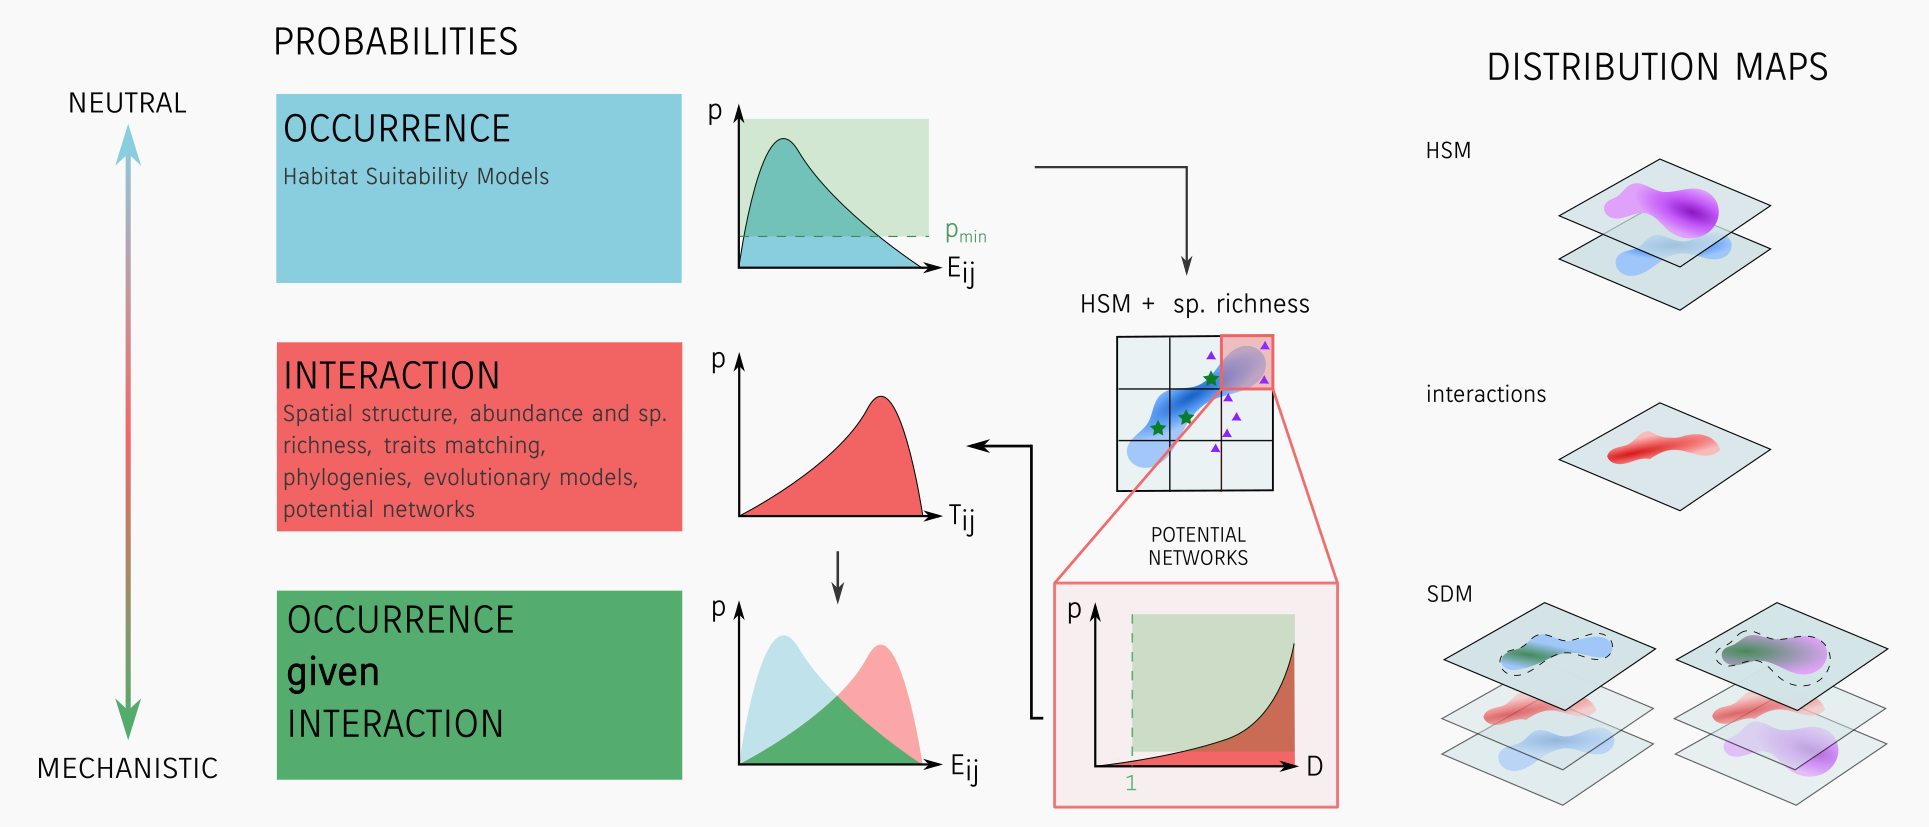
\includegraphics{figures/conc_fig4_chapX.png}
\caption{In the proposed workflow, probabilities of occurrence would be
updated by the probabilities of new interactions where the Habitat
Suitability Model suggests potential occurrence. For the sample sites
where a species is predicted to occur, but did not occur before, the
probability of this species to belong to a network where it has at least
one link would be calculated based on the species richness of those
cells. For the cells where the probability of having at least one link
is higher than 0 (or a given threshold, depending on the system), the
probability of interaction with important clades would then be assessed,
and finally this probability updates the probability of
occurrence.}\label{fig:synthesis}
}
\end{figure}

\hypertarget{i-potential-distribution-of-focal-species}{%
\subsubsection{(i) Potential distribution of focal
species}\label{i-potential-distribution-of-focal-species}}

A traditional habitat suitability model should be used as a first step
to assess the M+A space of the species (fig.~\ref{fig:bam}). The choice
of the best model will depend on a few criteria such as the nature and
quality of your data, and the processes you want to investigate, as
described in Guisan, Thuiller, and Zimmermann (2017) and Peterson et al.
(2012). A HSM will indicate where there are suitable habitats for the
species, which may include areas where the species was never sampled
before. These areas, the ``error'' of the model, should be the object of
assessment on the next steps since it is there where the unknown
information about interactions is. For each sample cell where the
species is predicted to occur, the value of known species richness can
be used to calculate potential networks with the addition of the focal
species.

\hypertarget{ii-potential-networks-based-on-species-richness}{%
\subsubsection{(ii) Potential networks based on species
richness}\label{ii-potential-networks-based-on-species-richness}}

The minimum and maximum number of links that are possible depends on how
many species share the same space (MacDonald, Banville, and Poisot
2020). Based on that, we can calculate the degree distributions that are
possible based on Maximum Entropy (HALP \textbf{francisbanville?})

\hypertarget{iii-potential-interactions-where-the-probability-of-a-degree-ge-1-is-not-null}{%
\subsubsection{\texorpdfstring{(iii) Potential interactions where the
probability of a degree \(\ge\) 1 is not
null}{(iii) Potential interactions where the probability of a degree \textbackslash ge 1 is not null}}\label{iii-potential-interactions-where-the-probability-of-a-degree-ge-1-is-not-null}}

For the cells where the focal species has at least one possible network
where its degree is \(\ge\) 1, we can proceed to investigate whether
this link is ecologically relevant. This can be done by sampling a
subset of species that occur and that could be important to that focal
species (either a competitor, a prey, a predator or a facilitator). Some
variables that can be important in this process are the phylogenetic or
the functional diversity, since they can help us subset the species pool
by evolutionary distance or ecological redundancy. Then the probability
of interaction can be calculated for the focal species and the subset of
species following the methods we discussed above, depending on the
nature of the data available at a macroecological scale. This analysis
should result on a spatial distribution of interaction probabilities for
each cell where the species where predicted to occur but was not sampled
before.

\hypertarget{iv-probability-of-occurrence-given-the-probability-of-interactions}{%
\subsubsection{(iv) Probability of occurrence given the probability of
interactions}\label{iv-probability-of-occurrence-given-the-probability-of-interactions}}

For those cells where we now have the probability of occurrence and
interaction, the probability of occurrence given the probability of
interaction is a new function \emph{h(x)}, which is a combination
between a function of probability of occurrence \emph{f(x)} and a
function of probability of interaction \emph{g(x)} eq.~\ref{eq:bayup}.\\
\begin{equation}\protect\hypertarget{eq:bayup}{}{h(x) = d(x)\left \lfloor \int f(x)-(\int f(x)-g(x))-(\int g(x)-f(x)) \right \rfloor}\label{eq:bayup}\end{equation}

TODO

Updating the probabilities of occurrence based on the probabilities of
interaction is a way to integrate biotic variables on species
distribution models as a separate step. We believe that this pathway can
simplify this intricate problem because it disentangles the complex
calculation of ecological interactions from the abiotic suitability
models. Both sides can be run in parallel, and in some cases the
probability of interaction does not need to be calculated every time a
model is run.

\begin{itemize}
\tightlist
\item
  What don't we have yet?
\item
  What are the roads never taken?
\item
  Where should we invest in order to achieve the best SDMs we can?
\item
  What are the most promising areas for development?
\end{itemize}

\hypertarget{references}{%
\subsection*{References}\label{references}}
\addcontentsline{toc}{subsection}{References}

\hypertarget{refs}{}
\begin{CSLReferences}{1}{0}
\leavevmode\hypertarget{ref-Afkhami2014MutEff}{}%
Afkhami, Michelle E., Patrick J. McIntyre, and Sharon Y. Strauss. 2014.
{``Mutualist-Mediated Effects on Species' Range Limits Across Large
Geographic Scales.''} \emph{Ecology Letters} 17 (10): 1265--73.
\url{https://doi.org/10.1111/ele.12332}.

\leavevmode\hypertarget{ref-Bar-Massada2017NonCoo}{}%
Bar-Massada, Avi, and Jonathan Belmaker. 2017. {``Non-Stationarity in
the Co-Occurrence Patterns of Species Across Environmental Gradients.''}
\emph{Journal of Ecology} 105 (2): 391--99.
\url{https://doi.org/10.1111/1365-2745.12713}.

\leavevmode\hypertarget{ref-Blanchet2020CooNot}{}%
Blanchet, F. Guillaume, Kevin Cazelles, and Dominique Gravel. 2020.
{``Co-Occurrence Is Not Evidence of Ecological Interactions.''}
\emph{Ecology Letters} 23 (7): 1050--63.
\url{https://doi.org/10.1111/ele.13525}.

\leavevmode\hypertarget{ref-Breiman2001RanFor}{}%
Breiman, Leo. 2001. {``Random Forests.''} \emph{Machine Learning} 45
(1): 5--32. \url{https://doi.org/10.1023/A:1010933404324}.

\leavevmode\hypertarget{ref-Bullock2000GeoSep}{}%
Bullock, James M., Rebecca J. Edwards, Peter D. Carey, and Rob J. Rose.
2000. {``Geographical Separation of Two Ulex Species at Three Spatial
Scales: Does Competition Limit Species' Ranges?''} \emph{Ecography} 23
(2): 257--71. \url{https://doi.org/10.1111/j.1600-0587.2000.tb00281.x}.

\leavevmode\hypertarget{ref-Cabral2017MecSim}{}%
Cabral, Juliano Sarmento, Luis Valente, and Florian Hartig. 2017.
{``Mechanistic Simulation Models in Macroecology and Biogeography:
State-of-Art and Prospects.''} \emph{Ecography} 40 (2): 267--80.
\url{https://doi.org/10.1111/ecog.02480}.

\leavevmode\hypertarget{ref-Callaghan2019ImpBig}{}%
Callaghan, Corey T., Jodi J. L. Rowley, William K. Cornwell, Alistair G.
B. Poore, and Richard E. Major. 2019. {``Improving Big Citizen Science
Data: Moving Beyond Haphazard Sampling.''} \emph{PLOS Biology} 17 (6):
e3000357. \url{https://doi.org/10.1371/journal.pbio.3000357}.

\leavevmode\hypertarget{ref-Canard2012EmeStr}{}%
Canard, Elsa, Nicolas Mouquet, Lucile Marescot, Kevin J. Gaston,
Dominique Gravel, and David Mouillot. 2012. {``Emergence of Structural
Patterns in Neutral Trophic Networks.''} \emph{PLOS ONE} 7 (8): e38295.
\url{https://doi.org/10.1371/journal.pone.0038295}.

\leavevmode\hypertarget{ref-Carnicer2009TemDyn}{}%
Carnicer, Jofre, Pedro Jordano, and Carlos J Melián. 2009. {``The
Temporal Dynamics of Resource Use by Frugivorous Birds: A Network
Approach.''} \emph{Ecology} 90 (7): 1958--70.

\leavevmode\hypertarget{ref-Cazelles2016IntBio}{}%
Cazelles, Kévin, Nicolas Mouquet, David Mouillot, and Dominique Gravel.
2016. {``On the Integration of Biotic Interaction and Environmental
Constraints at the Biogeographical Scale.''} \emph{Ecography} 39 (10):
921--31. \url{https://doi.org/10.1111/ecog.01714}.

\leavevmode\hypertarget{ref-Chesson2008IntPre}{}%
Chesson, Peter, and Jessica J. Kuang. 2008. {``The Interaction Between
Predation and Competition.''} \emph{Nature} 456 (7219): 235--38.
\url{https://doi.org/10.1038/nature07248}.

\leavevmode\hypertarget{ref-Coelho2017NeuBio}{}%
Coelho, Marco Túlio Pacheco, João Fabrício Mota Rodrigues, and Thiago F
Rangel. 2017. {``Neutral Biogeography of Phylogenetically Structured
Interaction Networks.''} \emph{Ecography} 40 (12): 1467--74.

\leavevmode\hypertarget{ref-Dallas2017PreCry}{}%
Dallas, Tad, Andrew W. Park, and John M. Drake. 2017. {``Predicting
Cryptic Links in Host-Parasite Networks.''} \emph{PLOS Computational
Biology} 13 (5): e1005557.
\url{https://doi.org/10.1371/journal.pcbi.1005557}.

\leavevmode\hypertarget{ref-Dallas2018ComTur}{}%
Dallas, Tad, and Timothée Poisot. 2018. {``Compositional Turnover in
Host and Parasite Communities Does Not Change Network Structure.''}
\emph{Ecography} 41 (9): 1534--42.
\url{https://doi.org/10.1111/ecog.03514}.

\leavevmode\hypertarget{ref-Dalsgaard2013HisCli}{}%
Dalsgaard, Bo, Kristian Trøjelsgaard, Ana M Martín González, David
Nogués-Bravo, Jeff Ollerton, Theodora Petanidou, Brody Sandel, et al.
2013. {``Historical Climate-Change Influences Modularity and Nestedness
of Pollination Networks.''} \emph{Ecography} 36 (12): 1331--40.

\leavevmode\hypertarget{ref-Davies2011PhyDiv}{}%
Davies, T Jonathan, and Lauren B Buckley. 2011. {``Phylogenetic
Diversity as a Window into the Evolutionary and Biogeographic Histories
of Present-Day Richness Gradients for Mammals.''} \emph{Philos. Trans.
R. Soc. Lond. B Biol. Sci.} 366 (1576): 2414--25.

\leavevmode\hypertarget{ref-Dattilo2020SpeDri}{}%
Dáttilo, Wesley, Nathalia Barrozo-Chávez, Andrés Lira-Noriega, Roger
Guevara, Fabricio Villalobos, Diego Santiago-Alarcon, Frederico Siqueira
Neves, Thiago Izzo, and Sérvio Pontes Ribeiro. 2020. {``Species-Level
Drivers of Mammalian Ectoparasite Faunas.''} \emph{Journal of Animal
Ecology} 89 (8): 1754--65.
\url{https://doi.org/10.1111/1365-2656.13216}.

\leavevmode\hypertarget{ref-Desjardins-Proulx2017EcoInt}{}%
Desjardins-Proulx, Philippe, Idaline Laigle, Timothée Poisot, and
Dominique Gravel. 2017. {``Ecological Interactions and the Netflix
Problem.''} \emph{PeerJ} 5 (August): e3644.
\url{https://doi.org/10.7717/peerj.3644}.

\leavevmode\hypertarget{ref-Dunne2002NetStr}{}%
Dunne, Jennifer A., Richard J. Williams, and Neo D. Martinez. 2002.
{``Network Structure and Biodiversity Loss in Food Webs: Robustness
Increases with Connectance.''} \emph{Ecology Letters} 5 (4): 558--67.
\url{https://doi.org/10.1046/j.1461-0248.2002.00354.x}.

\leavevmode\hypertarget{ref-Elmasri2020HieBay}{}%
Elmasri, Mohamad, Maxwell J. Farrell, T. Jonathan Davies, and David A.
Stephens. 2020. {``A Hierarchical Bayesian Model for Predicting
Ecological Interactions Using Scaled Evolutionary Relationships.''}
\emph{Annals of Applied Statistics} 14 (1): 221--40.
\url{https://doi.org/10.1214/19-AOAS1296}.

\leavevmode\hypertarget{ref-Ferrier2006SpaMod}{}%
Ferrier, Simon, and Antoine Guisan. 2006. {``Spatial Modelling of
Biodiversity at the Community Level.''} \emph{Journal of Applied
Ecology} 43 (3): 393--404.
\url{https://doi.org/10.1111/j.1365-2664.2006.01149.x}.

\leavevmode\hypertarget{ref-Galiana2018SpaSca}{}%
Galiana, Nuria, Miguel Lurgi, Bernat Claramunt-López, Marie-Josée
Fortin, Shawn Leroux, Kevin Cazelles, Dominique Gravel, and José M.
Montoya. 2018. {``The Spatial Scaling of Species Interaction
Networks.''} \emph{Nature Ecology \& Evolution} 2 (5): 782--90.
\url{https://doi.org/10.1038/s41559-018-0517-3}.

\leavevmode\hypertarget{ref-Gbi}{}%
{``GBIF.''} n.d. https://www.gbif.org/.

\leavevmode\hypertarget{ref-Godsoe2012HowSpe}{}%
Godsoe, William, and Luke J. Harmon. 2012. {``How Do Species
Interactions Affect Species Distribution Models?''} \emph{Ecography} 35
(9): 811--20. \url{https://doi.org/10.1111/j.1600-0587.2011.07103.x}.

\leavevmode\hypertarget{ref-Godsoe2017IntBio}{}%
Godsoe, William, Jill Jankowski, Robert D. Holt, and Dominique Gravel.
2017. {``Integrating Biogeography with Contemporary Niche Theory.''}
\emph{Trends in Ecology and Evolution} 32 (7): 488--99.
\url{https://doi.org/10.1016/j.tree.2017.03.008}.

\leavevmode\hypertarget{ref-Gomez2010EcoInt}{}%
Gómez, José M., Miguel Verdú, and Francisco Perfectti. 2010.
{``Ecological Interactions Are Evolutionarily Conserved Across the
Entire Tree of Life.''} \emph{Nature} 465 (7300): 918--21.
\url{https://doi.org/10.1038/nature09113}.

\leavevmode\hypertarget{ref-Gravel2011TroThe}{}%
Gravel, Dominique, François Massol, Elsa Canard, David Mouillot, and
Nicolas Mouquet. 2011. {``Trophic Theory of Island Biogeography.''}
\emph{Ecology Letters} 14 (10): 1010--16.
\url{https://doi.org/10.1111/j.1461-0248.2011.01667.x}.

\leavevmode\hypertarget{ref-Guimaraes2020StrEco}{}%
Guimarães, Paulo R. 2020. {``The Structure of Ecological Networks Across
Levels of Organization.''} \emph{Annual Review of Ecology, Evolution,
and Systematics} 51 (1): 433--60.
\url{https://doi.org/10.1146/annurev-ecolsys-012220-120819}.

\leavevmode\hypertarget{ref-Guisan2006MakBet}{}%
Guisan, Antoine, Anthony Lehmann, Simon Ferrier, Mike Austin, Jacob Mc.
C. Overton, Richard Aspinall, and Trevor Hastie. 2006. {``Making Better
Biogeographical Predictions of Species' Distributions.''} \emph{Journal
of Applied Ecology} 43 (3): 386--92.
\url{https://doi.org/10.1111/j.1365-2664.2006.01164.x}.

\leavevmode\hypertarget{ref-Guisan2017HabSui}{}%
Guisan, Antoine, Wilfried Thuiller, and Niklaus E. Zimmermann. 2017.
\emph{Habitat Suitability and Distribution Models: With Applications in
R}. Ecology, Biodiversity and Conservation. Cambridge: Cambridge
University Press. \url{https://doi.org/10.1017/9781139028271}.

\leavevmode\hypertarget{ref-Guisan2000PreHab}{}%
Guisan, Antoine, and Niklaus E. Zimmermann. 2000. {``Predictive Habitat
Distribution Models in Ecology.''} \emph{Ecological Modelling} 135 (2):
147--86. \url{https://doi.org/10.1016/S0304-3800(00)00354-9}.

\leavevmode\hypertarget{ref-Harmon2010EarBur}{}%
Harmon, Luke J., Jonathan B. Losos, T. Jonathan Davies, Rosemary G.
Gillespie, John L. Gittleman, W. Bryan Jennings, Kenneth H. Kozak, et
al. 2010. {``Early Bursts of Body Size and Shape Evolution Are Rare in
Comparative Data.''} \emph{Evolution} 64 (8): 2385--96.
\url{https://doi.org/10.1111/j.1558-5646.2010.01025.x}.

\leavevmode\hypertarget{ref-Hellmann2012InfSpe}{}%
Hellmann, Jessica J., Kirsten M. Prior, and Shannon L. Pelini. 2012.
{``The Influence of Species Interactions on Geographic Range Change
Under Climate Change.''} \emph{Annals of the New York Academy of
Sciences} 1249 (February): 18--28.
\url{https://doi.org/10.1111/j.1749-6632.2011.06410.x}.

\leavevmode\hypertarget{ref-Hortal2015SevSho}{}%
Hortal, Joaquín, Francesco de Bello, José Alexandre F. Diniz-Filho,
Thomas M. Lewinsohn, Jorge M. Lobo, and Richard J. Ladle. 2015. {``Seven
Shortfalls That Beset Large-Scale Knowledge of Biodiversity.''}
\emph{Annual Review of Ecology, Evolution, and Systematics} 46 (1):
523--49. \url{https://doi.org/10.1146/annurev-ecolsys-112414-054400}.

\leavevmode\hypertarget{ref-Ingram2012WheSho}{}%
Ingram, T., L. J. Harmon, and J. B. Shurin. 2012. {``When Should We
Expect Early Bursts of Trait Evolution in Comparative Data? Predictions
from an Evolutionary Food Web Model.''} \emph{Journal of Evolutionary
Biology} 25 (9): 1902--10.
\url{https://doi.org/10.1111/j.1420-9101.2012.02566.x}.

\leavevmode\hypertarget{ref-Jordano2016SamNet}{}%
Jordano, Pedro. 2016. {``Sampling Networks of Ecological
Interactions.''} \emph{Functional Ecology} 30 (12): 1883--93.
\url{https://doi.org/10.1111/1365-2435.12763}.

\leavevmode\hypertarget{ref-JorgeSoberon2007GriElt}{}%
Jorge Soberón. 2007. {``Grinnellian and Eltonian Niches and Geographic
Distributions of Species.''} \emph{Ecology Letters} 10 (12): 1115--23.
\url{https://doi.org/10.1111/j.1461-0248.2007.01107.x}.

\leavevmode\hypertarget{ref-Konig2019BioDat}{}%
König, Christian, Patrick Weigelt, Julian Schrader, Amanda Taylor, Jens
Kattge, and Holger Kreft. 2019. {``Biodiversity Data Integrationthe
Significance of Data Resolution and Domain.''} \emph{PLOS Biology} 17
(3): e3000183. \url{https://doi.org/10.1371/journal.pbio.3000183}.

\leavevmode\hypertarget{ref-MacArthur1967TheIsl}{}%
MacArthur, Robert H., and Edward O. Wilson. 1967. \emph{The Theory of
Island Biogeography}. Princeton University Press.

\leavevmode\hypertarget{ref-MacDonald2020RevLin}{}%
MacDonald, Arthur Andrew Meahan, Francis Banville, and Timothée Poisot.
2020. {``Revisiting the Links-Species Scaling Relationship in Food
Webs.''} \emph{Patterns} 1 (0).
\url{https://doi.org/10.1016/j.patter.2020.100079}.

\leavevmode\hypertarget{ref-MartinGonzalez2015MacPhy}{}%
Martín González, Ana M., Bo Dalsgaard, David Nogués-Bravo, Catherine H.
Graham, Matthias Schleuning, Pietro K. Maruyama, Stefan Abrahamczyk, et
al. 2015. {``The Macroecology of Phylogenetically Structured
Hummingbird-Plant Networks.''} \emph{Global Ecology and Biogeography} 24
(11): 1212--24. \url{https://doi.org/10.1111/geb.12355}.

\leavevmode\hypertarget{ref-Memmott2004TolPol}{}%
Memmott, J., N. M. Waser, and M. V. Price. 2004. {``Tolerance of
Pollination Networks to Species Extinctions.''} \emph{Proceedings of the
Royal Society B: Biological Sciences} 271 (1557): 2605--11.
\url{https://doi.org/10.1098/rspb.2004.2909}.

\leavevmode\hypertarget{ref-Muola2010AssPla}{}%
Muola, Anne, Pia Mutikainen, Marianna Lilley, Liisa Laukkanen, Juha
Pekka Salminen, and Roosa Leimu. 2010. {``Associations of Plant Fitness,
Leaf Chemistry, and Damage Suggest Selection Mosaic in Plant-Herbivore
Interactions.''} \emph{Ecology}.
\url{https://doi.org/10.1890/09-0589.1}.

\leavevmode\hypertarget{ref-Olden2008MacLea}{}%
Olden, Julian, Joshua Lawler, and N. Poff. 2008. {``Machine Learning
Methods Without Tears: A Primer for Ecologists.''} \emph{The Quarterly
Review of Biology} 83 (July): 171--93.
\url{https://doi.org/10.1086/587826}.

\leavevmode\hypertarget{ref-Peralta2016MerEvo}{}%
Peralta, Guadalupe. 2016. {``Merging Evolutionary History into Species
Interaction Networks.''} \emph{Functional Ecology} 30 (12): 1917--25.
\url{https://doi.org/10.1111/1365-2435.12669}.

\leavevmode\hypertarget{ref-Peterson2012EcoNic}{}%
Peterson, A. Townsend, Jorge Soberón, Richard G. Pearson, Robert P.
Anderson, Enrique Martínez-Meyer, Miguel Nakamura, and Miguel Bastos
Araújo. 2012. \emph{Ecological Niches and Geographic Distributions}.
\emph{Choice Reviews Online}. Vol. 49.
\url{https://doi.org/10.5860/CHOICE.49-6266}.

\leavevmode\hypertarget{ref-Phillips2006MaxEnt}{}%
Phillips, Steven J., Robert P. Anderson, and Robert E. Schapire. 2006.
{``Maximum Entropy Modeling of Species Geographic Distributions.''}
\emph{Ecological Modelling} 190 (3): 231--59.
\url{https://doi.org/10.1016/j.ecolmodel.2005.03.026}.

\leavevmode\hypertarget{ref-Pichler2019MacLea}{}%
Pichler, Maximilian, Virginie Boreux, Alexandra-Maria Klein, Matthias
Schleuning, and Florian Hartig. {``Machine Learning Algorithms to Infer
Trait-Matching and Predict Species Interactions in Ecological
Networks.''} \emph{Methods in Ecology and Evolution} 11 (2): 281--93.
\url{https://doi.org/10.1111/2041-210X.13329}.

\leavevmode\hypertarget{ref-Pocock2015BioRec}{}%
Pocock, Michael J. O., Helen E. Roy, Chris D. Preston, and David B. Roy.
2015. {``The Biological Records Centre: A Pioneer of Citizen Science.''}
\emph{Biological Journal of the Linnean Society} 115 (3): 475--93.
\url{https://doi.org/10.1111/bij.12548}.

\leavevmode\hypertarget{ref-Poisot2016ManMak}{}%
Poisot, Timothée, Benjamin Baiser, Jennifer A Dunne, Sonia Kéfi,
François Massol, Nicolas Mouquet, Tamara N Romanuk, Daniel B Stouffer,
Spencer A Wood, and Dominique Gravel. 2016. {``Mangal - Making
Ecological Network Analysis Simple.''} \emph{Ecography} 39 (4): 384--90.

\leavevmode\hypertarget{ref-Poisot2020EnvBia}{}%
Poisot, Timothée, Gabriel Bergeron, Kevin Cazelles, Tad Dallas,
Dominique Gravel, Andrew Macdonald, Benjamin Mercier, Clément Violet,
and Steve Vissault. 2020. {``Environmental Biases in the Study of
Ecological Networks at the Planetary Scale.''} \emph{bioRxiv}, January.
\url{https://doi.org/10.1101/2020.01.27.921429}.

\leavevmode\hypertarget{ref-Poisot2016StrPro}{}%
Poisot, Timothée, Alyssa R Cirtwill, Kévin Cazelles, Dominique Gravel,
Marie Josée Fortin, and Daniel B Stouffer. 2016. {``The Structure of
Probabilistic Networks.''} \emph{Methods in Ecology and Evolution} 7
(3): 303--12. \url{https://doi.org/10.1111/2041-210X.12468}.

\leavevmode\hypertarget{ref-Poisot2017HosPar}{}%
Poisot, Timothée, Cynthia Guéveneux-Julien, Marie Josée Fortin,
Dominique Gravel, and Pierre Legendre. 2017. {``Hosts, Parasites and
Their Interactions Respond to Different Climatic Variables.''}
\emph{Global Ecology and Biogeography} 26 (8): 942--51.
\url{https://doi.org/10.1111/geb.12602}.

\leavevmode\hypertarget{ref-Poisot2016HowEco}{}%
Poisot, Timothée, and Daniel Stouffer. 2016. {``How Ecological Networks
Evolve.''} \emph{bioRxiv}, no. Jablonski 2008: 071993.
\url{https://doi.org/10.1101/071993}.

\leavevmode\hypertarget{ref-Poisot2014SpeWhy}{}%
Poisot, Timothée, Daniel B. Stouffer, and Dominique Gravel. 2014.
{``Beyond Species: Why Ecological Interaction Networks Vary Through
Space and Time.''} \emph{Oikos} 124 (3): 243--51.
\url{https://doi.org/10.1111/oik.01719}.

\leavevmode\hypertarget{ref-Pollock2014UndCoo}{}%
Pollock, Laura J., Reid Tingley, William K. Morris, Nick Golding, Robert
B. O'Hara, Kirsten M. Parris, Peter A. Vesk, and Michael A. McCarthy.
2014. {``Understanding Co-Occurrence by Modelling Species Simultaneously
with a Joint Species Distribution Model (JSDM).''} \emph{Methods in
Ecology and Evolution} 5 (5): 397--406.
\url{https://doi.org/10.1111/2041-210X.12180}.

\leavevmode\hypertarget{ref-Rall2012UniTem}{}%
Rall, B. C., U. Brose, M. Hartvig, G. Kalinkat, F. Schwarzmuller, O.
Vucic-Pestic, and O. L. Petchey. 2012. {``Universal Temperature and
Body-Mass Scaling of Feeding Rates.''} \emph{Philosophical Transactions
of the Royal Society B: Biological Sciences} 367 (1605): 2923--34.
\url{https://doi.org/10.1098/rstb.2012.0242}.

\leavevmode\hypertarget{ref-Ramos-Jiliberto2012TopPla}{}%
Ramos-Jiliberto, Rodrigo, Fernanda S. Valdovinos, Pablo Moisset de
Espanés, and José D. Flores. 2012. {``Topological Plasticity Increases
Robustness of Mutualistic Networks.''} \emph{Journal of Animal Ecology}
81 (4): 896--904.
\url{https://doi.org/10.1111/j.1365-2656.2012.01960.x}.

\leavevmode\hypertarget{ref-Rangel2012LabEco}{}%
Rangel, Thiago Fernando, and Rafael Dias Loyola. 2012. {``Labeling
Ecological Niche Models.''} \emph{Natureza \& Conservação} 10 (2):
119--26. \url{https://doi.org/10.4322/natcon.2012.030}.

\leavevmode\hypertarget{ref-Riva2016ExpEvo}{}%
Riva, Giulio V. Dalla, and Daniel B. Stouffer. 2016. {``Exploring the
Evolutionary Signature of Food Webs' Backbones Using Functional
Traits.''} \emph{Oikos} 125 (4): 446--56.
\url{https://doi.org/10.1111/oik.02305}.

\leavevmode\hypertarget{ref-Roy2016FocPla}{}%
Roy, Helen E., Elizabeth Baxter, Aoine Saunders, and Michael J. O.
Pocock. 2016. {``Focal Plant Observations as a Standardised Method for
Pollinator Monitoring: Opportunities and Limitations for Mass
Participation Citizen Science.''} \emph{PLOS ONE} 11 (3): e0150794.
\url{https://doi.org/10.1371/journal.pone.0150794}.

\leavevmode\hypertarget{ref-Ryan2018RolCit}{}%
Ryan, S. F., N. L. Adamson, A. Aktipis, L. K. Andersen, R. Austin, L.
Barnes, M. R. Beasley, et al. 2018. {``The Role of Citizen Science in
Addressing Grand Challenges in Food and Agriculture Research.''}
\emph{Proceedings of the Royal Society B: Biological Sciences} 285
(1891). \url{https://doi.org/10.1098/rspb.2018.1977}.

\leavevmode\hypertarget{ref-Sanders2012IndCom}{}%
Sanders, Dirk, and F. J.Frank Van Veen. 2012. {``Indirect Commensalism
Promotes Persistence of Secondary Consumer Species.''} \emph{Biology
Letters} 8 (6): 960--63. \url{https://doi.org/10.1098/rsbl.2012.0572}.

\leavevmode\hypertarget{ref-Sebastian-Gonzalez2015MacTre}{}%
Sebastián-González, Esther, Bo Dalsgaard, Brody Sandel, and Paulo R
Guimarães. 2015. {``Macroecological Trends in Nestedness and Modularity
of Seed-Dispersal Networks: Human Impact Matters.''} \emph{Global
Ecology and Biogeography} 24 (3): 293--303.

\leavevmode\hypertarget{ref-Siren2020IntRan}{}%
Sirén, Alexej P. K., and Toni Lyn Morelli. 2020. {``Interactive
Range-Limit Theory (iRLT): An~Extension for Predicting Range Shifts.''}
\emph{Journal of Animal Ecology} 89 (4): 940--54.
\url{https://doi.org/10.1111/1365-2656.13150}.

\leavevmode\hypertarget{ref-Soberon2009NicDis}{}%
Soberón, Jorge, and Miguel Nakamura. 2009. {``Niches and Distributional
Areas: Concepts, Methods, and Assumptions.''} \emph{Proceedings of the
National Academy of Sciences} 106 (Supplement 2): 19644--50.
\url{https://doi.org/10.1073/pnas.0901637106}.

\leavevmode\hypertarget{ref-Staniczenko2017LinMac}{}%
Staniczenko, Phillip P. A., Prabu Sivasubramaniam, K. Blake Suttle, and
Richard G. Pearson. 2017. {``Linking Macroecology and Community Ecology:
Refining Predictions of Species Distributions Using Biotic Interaction
Networks.''} \emph{Ecology Letters} 20 (6): 693--707.
\url{https://doi.org/10.1111/ele.12770}.

\leavevmode\hypertarget{ref-Svenning2014InfInt}{}%
Svenning, Jens Christian, Dominique Gravel, Robert D. Holt, Frank M.
Schurr, Wilfried Thuiller, Tamara Münkemüller, Katja H. Schiffers, et
al. 2014. {``The Influence of Interspecific Interactions on Species
Range Expansion Rates.''} \emph{Ecography} 37 (12): 1198--1209.
\url{https://doi.org/10.1111/j.1600-0587.2013.00574.x}.

\leavevmode\hypertarget{ref-Trojelsgaard2013MacPol}{}%
Trøjelsgaard, Kristian, and Jens M Olesen. 2013. {``Macroecology of
Pollination Networks.''} \emph{Global Ecology and Biogeography} 22 (2):
149--62.

\leavevmode\hypertarget{ref-Tylianakis2017EcoNet}{}%
Tylianakis, Jason M., and Rebecca J. Morris. 2017. {``Ecological
Networks Across Environmental Gradients.''} \emph{Annual Review of
Ecology, Evolution, and Systematics} 48 (1):
annurev-ecolsys-110316-022821.
\url{https://doi.org/10.1146/annurev-ecolsys-110316-022821}.

\leavevmode\hypertarget{ref-Wisz2013RolBio}{}%
Wisz, Mary Susanne, Julien Pottier, W Daniel Kissling, Loïc Pellissier,
Jonathan Lenoir, Christian F Damgaard, Carsten F Dormann, et al. 2013.
{``The Role of Biotic Interactions in Shaping Distributions and Realised
Assemblages of Species: Implications for Species Distribution
Modelling.''} \emph{Biological Reviews of the Cambridge Philosophical
Society} 88 (1): 15--30.
\url{https://doi.org/10.1111/j.1469-185X.2012.00235.x}.

\leavevmode\hypertarget{ref-Wolin1984ModFac}{}%
Wolin, Carole L., and Lawrence R. Lawlor. 1984. {``Models of Facultative
Mutualism: Density Effects.''} \emph{The American Naturalist} 124 (6):
843--62. \url{https://doi.org/10.1086/284320}.

\leavevmode\hypertarget{ref-XiaoFu2019LinPre}{}%
Xiao Fu, Eugene Seo, Justin Clarke, and Rebecca A. Hutchinson. 2019.
{``Link Prediction Under Imperfect Detection: Collaborative Filtering
for Ecological Networks.''} \emph{IEEE Transactions on Knowledge \& Data
Engineering}, no. 01 (December).
\url{https://doi.org/10.1109/TKDE.2019.2962031}.

\leavevmode\hypertarget{ref-Zurell2020TesSpe}{}%
Zurell, Damaris, Niklaus E. Zimmermann, Helge Gross, Andri
Baltensweiler, Thomas Sattler, and Rafael O. Wüest. 2020. {``Testing
Species Assemblage Predictions from Stacked and Joint Species
Distribution Models.''} \emph{Journal of Biogeography} 47 (1): 101--13.
\url{https://doi.org/10.1111/jbi.13608}.

\end{CSLReferences}

\end{document}
